\chapter{Metodología}
\label{chap:metodologia}

\section{Propuesta de simulación}

En esta sección, previa a la implementación, se describe el escenario diseñado para el desarrollo del trabajo.

El objetivo principal de este entorno es servir como material práctico de entrenamiento para analistas de seguridad, permitiendo la reconstrucción de un incidente realista a partir de un conjunto controlado de artefactos. Para ello, se define la infraestructura de la organización víctima y se pone a disposición el conjunto completo de evidencias generadas durante la simulación del incidente.

El propósito del analista es reconstruir la cadena completa del ataque mediante el análisis de dichos artefactos, identificando las técnicas empleadas y correlacionando la información disponible. Para estructurar este proceso, el trabajo se organiza en dos subsecciones complementarias:

\subsection{El Incidente \ref{chap:incidente}}
En este capítulo se describe de forma secuencial la actividad del atacante, incluyendo sus objetivos, las técnicas MITRE ATT\&CK asociadas y las evidencias donde pueden observarse.

\subsection{Red Team Notes \ref{chap:red-team}}
Este capítulo ofrece una visión complementaria desde la perspectiva del atacante, detallando las acciones realizadas durante la intrusión y los procedimientos empleados para comprometer el sistema.

\section{Descripción del Atacante}

En este trabajo no se modela un adversario real ni se replica el comportamiento de un APT existente. En su lugar, se diseña un atacante ad hoc, construido específicamente para este escenario con fines didácticos. Este enfoque permite ajustar de forma controlada sus tácticas, técnicas y decisiones operativas para alinearlas con los objetivos formativos del ejercicio.

\section{Descripción del Ataque (Resumen Ejecutivo)}

\begin{figure}[h!]
    \centering
    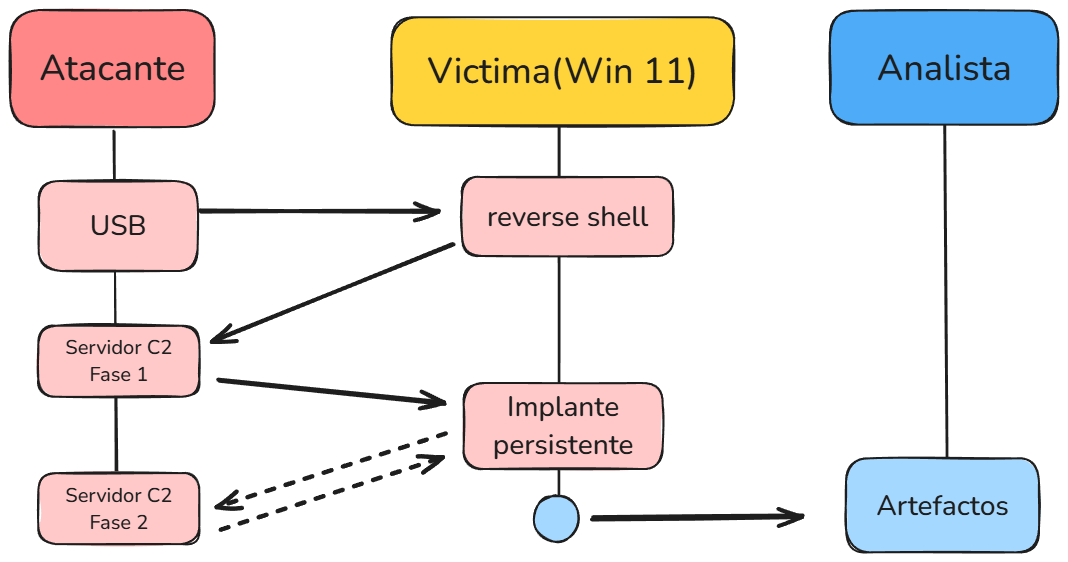
\includegraphics[width=0.8\textwidth]{figures/ataque.png}
    \caption{Visión general del escenario: el atacante obtiene acceso inicial mediante un dispositivo físico (fase 1) y despliega un implante que mantiene comunicación cifrada con su infraestructura C2 (fase 2).}
    \label{fig:ataque}
\end{figure}

El escenario propuesto reproduce un ataque estructurado en dos fases, diseñado para simular el comportamiento de un adversario realista.

En la primera fase, el atacante obtiene acceso inicial al sistema víctima mediante el uso de un dispositivo físico que le permite ejecutar código de forma inmediata. A partir de este punto de entrada, establece una conexión remota hacia su infraestructura externa, desde la cual realiza un reconocimiento básico del sistema y prepara la siguiente etapa del ataque.

En la segunda fase, el adversario despliega su componente principal, diseñado para operar de forma persistente y con baja visibilidad dentro del sistema. Este componente establece mecanismos de persistencia, amplía las capacidades de control remoto y se integra en procesos legítimos del sistema con el objetivo de dificultar su detección. A partir de este momento, el atacante puede realizar acciones más avanzadas, como el análisis del entorno, la escalada de privilegios, el movimiento lateral o la exfiltración de información.

\subsection*{Infraestructura de la víctima}

Como base del entorno corporativo se utiliza \textbf{GOAD-Light}, una versión reducida del laboratorio GOAD orientada a entornos de Active Directory vulnerables. Este entorno proporciona un dominio Windows preconfigurado, servicios esenciales y múltiples debilidades intencionadas que permiten simular técnicas reales de compromiso y movimiento lateral.

Las características completas del entorno GOAD-Light están documentadas por sus autores \cite{goad-light}.

Dentro del dominio se incluye una \textbf{estación de trabajo Windows 11}, completamente actualizada y con las protecciones de seguridad nativas habilitadas. Esta máquina actúa como punto de entrada inicial del ataque y como principal superficie de interacción con el usuario víctima.

Con el objetivo de aumentar la visibilidad del análisis forense y enriquecer el conjunto de artefactos disponibles, se incorporan dos componentes adicionales:

\begin{itemize}
    \item \textbf{Suricata}: desplegado para la monitorización del tráfico de red, permitiendo detectar y correlacionar conexiones sospechosas, tráfico de comando y control (\textit{C2}) y patrones de actividad maliciosa.
    
    \item \textbf{Sysmon}: instalado en la estación de trabajo para generar telemetría avanzada de eventos en Windows, incluyendo creación de procesos, carga de DLLs, conexiones de red y modificaciones en el registro, facilitando la reconstrucción temporal del ataque.
\end{itemize}

\subsection{Recopilación de evidencias}

En el siguiente enlace se encuentran todas las evidencias recopiladas del incidente:

\begin{center}
\href{https://drive.google.com/drive/folders/18eekh9kx51psuuTZ_nHl3NHEQLJb7zRV?usp=drive_link}{\textbf{Carpeta de evidencias del incidente}}
\end{center}

Cada carpeta corresponde a un equipo de la organización y lleva su nombre. Dentro de cada una se incluyen todos los artefactos adquiridos.

Los artefactos consisten en un volcado de la memoria RAM del equipo y otros elementos relevantes obtenidos durante la adquisición.

La recopilación se ha realizado con la herramienta \textbf{KAPE}, utilizando archivos \texttt{.tkape}. Estos archivos definen qué artefactos se recolectan, desde qué rutas y con qué reglas. Una explicación detallada sobre qué es un Target de KAPE puede consultarse en \cite{kape-targets}.

En este caso, se han utilizado los siguientes Targets:

\begin{itemize}
    \item \texttt{\string!SANS\_Triage} \cite{sans_triage_kape}
    \item \texttt{EventLogs} \cite{eventlogs_kape}
\end{itemize}

\subsection{Cómo utilizar este recurso}

Este recurso está pensado para servir como guía de apoyo durante el análisis del incidente y como material de referencia técnica para comprender en detalle cómo se desarrolló el ataque.

El contenido se organiza en dos bloques complementarios:

\begin{itemize}
    \item \textbf{Capítulo \ref{chap:background}: Background.}  
    Vocabulario técnico e instituciones sobre las que se apoya el contenido del trabajo.

    \item \textbf{Capítulo \ref{chap:incidente}: Reconstrucción del ciberataque.}  
    Presenta una visión estructurada del ataque, mapeando cada acción del adversario con las técnicas MITRE ATT\&CK aplicadas y con los artefactos del sistema víctima donde podría encontrarse evidencia relevante. Este bloque está orientado a facilitar el trabajo del analista DFIR durante el proceso de correlación y reconstrucción de los hechos.

    \item \textbf{Capítulo \ref{chap:red-team}: Red Team Notes.}  
    Describe el ataque desde el punto de vista del adversario, explicando el razonamiento, las decisiones técnicas y los procedimientos utilizados en cada fase. Ofrece una visión interna del flujo del ataque y del funcionamiento de cada componente ofensivo.
\end{itemize}

El proyecto está diseñado para que el analista pueda avanzar de forma autónoma utilizando únicamente las evidencias del caso. Si en algún momento necesita orientación sobre dónde buscar rastros de una técnica, puede consultar el Capítulo \ref{chap:incidente}. Si, en cambio, desea entender en profundidad por qué el atacante actuó de una determinada manera o cómo funciona una técnica concreta, puede acudir al Capítulo \ref{chap:red-team}, donde se detalla su implementación desde la perspectiva del red team.

\begin{center}
\fbox{
    \begin{minipage}{0.75\textwidth}
        \centering
        \textbf{Si deseas analizar el caso sin spoilers, no continúes leyendo.}
    \end{minipage}
}
\end{center}